\documentclass[professionalfonts, xcolor={usenames,svgnames,x11names,table}]{beamer}

\usetheme{SBUclass}
\usepackage[charter]{mathdesign}
\usepackage[scaled]{helvet}

\usepackage{mypackages}

\title{\texorpdfstring{Language \& Technology}{Language and Technology}}
\subtitle{Syllabus}
\author{Al{\"e}na Aks{\"e}nova \& Aniello De Santo}
\institute{Stony Brook University\\\texttt{alena.aksenova@stonybrook.edu}\\\texttt{aniello.desanto@stonybrook.edu}}
\date{Jan 28, 2019}


\begin{document}
\unnumbered{
\begin{frame}
	\titlepage
\end{frame}
}

\begin{frame}{Organizational Information}
    \begin{center}
        \begin{tabular}{r@{\hspace{2em}}l}
            \textbf{Course}            & Language and Technology\\
            \textbf{Course\#}          & LIN 120\\
            \textbf{Room}              & Humanities 1006\\
            \textbf{Time - Session 1}              & MW 10:00--10:53\\ 
              \textbf{Time  - Session 2}              & MW 11:00--11:53\\ 
            \textbf{Website}           & Cocalc and Blackboard\\[12pt]
                    \end{tabular}
     \begin{tabular}{r@{\hspace{2em}}ll}
            \textbf{Instructor}        & Al{\"e}na Aks{\"e}nova & Aniello De Santo\\
            \textbf{Office hours}      & W 1:00 -- 4:00 &  M 12:00 -- 2:00\\
                                        & &F 12:00--1:00\\
            \textbf{Office}            & SBS N210 & SBS N232\\[12pt] 
                 %       \textbf{Email}             & \url{alena.aksenova@stonybrook.edu} &  \url{aniello.desanto@stonybrook.edu}  \\
        \end{tabular}
     \begin{tabular}{r@{\hspace{2em}}l}
            \textbf{TAs}               & Pablo Lopes Alonso \& Kalina Kostyszyn \&  Jun Lyu\\
            \textbf{Undergraduate TAs} & Jessica Ju, Zhan Peng Zheng,  Cody St. Clair \\ 
 & Kathryn Chen, Elizabeth Lei, Jack Jiang\\
        \end{tabular}
    \end{center}

    See the Blackboard course page for more details and announcements.
\end{frame}


\begin{frame}{Bulletin Description}
    \small

    An introduction to how computers process language and solve language-related tasks. This course discusses the language technologies of our daily life --- spam filtering, machine translation, and many more --- and shows how they work under the hood. The course explores a variety of issues: Why do computers do well in some areas (spell checking) yet fail miserably in others (essay grading)? Will we ever have perfectly fluent AIs as depicted in science fiction? And how will these technological advances impact the role of language in our society? Students will also acquire basic programming skills and write scripts for simple language tasks. No previous training in mathematics or computer science required.    

    \textbf{SBC:} TECH

    3 credits
\end{frame}

\begin{frame}{An Experiment}
    \begin{enumerate}
        \item Open some chat or messaging app on your phone.
        \item Don't type anything.
        \item Instead, click the second word suggestion\\
              (the one in the middle).
        \item Keep doing this.
        \item Did you get a reasonable sentence of English?
    \end{enumerate}

    \visible<2>{
        \begin{quote}
            I am a beautiful person who is the best of luck to you by the way to get the best of luck to you by the way to get the best of luck to you by the way to get the \ldots
        \end{quote}
        }
\end{frame}

\begin{frame}{The Big Take-Home Message}
    \begin{center}
        \begin{tikzpicture}
            \node[draw=Red3,fill=Red3!25,thick,
                  font=\LARGE\bfseries, align=center,
                  inner sep=1em] at (0,0) %
                {Current language technology is mostly\\ smoke and mirrors};
        \end{tikzpicture}
    \end{center}
\end{frame}

\begin{frame}{Questions and Topics}
    \begin{itemize}
        \item How do computers process language?
        \item Why do they succeed in some areas (spell checker, spam filter),\\
            yet fail miserably in others (translation, poetry)?
        \item Will we ever have conversant AIs as depicted in science fiction\\
            (2001, Star Trek, Blade Runner, Her, Ex Machina, System Shock)?
        \item Can computers provide new answers to long-standing questions of linguistics and philology?
        \item How are language communities affected by these new technologies?
    \end{itemize}
\end{frame}

\begin{frame}{Teaching Goals}
    \begin{itemize}
        \item \textbf{Basics of Programming and Computer Science}
            \begin{itemize}
                \item understand the importance of algorithms and data structures
                \item conceptualize linguistic problems in computational terms
                \item basic programming skills in Python
            \end{itemize}
        \pause
        \item \textbf{Cognitive Science}
            \begin{itemize}
                \item familiarity with notions of artificial intelligence
                \item understand how and why humans and computers\\
                    differ in their linguistic abilities
            \end{itemize}
        \pause
        \item \textbf{Digital Humanities and Social Science}
            \begin{itemize}
                \item work with text corpora
                \item use computational tools for humanities\\
                    (stylistic analysis, tracking social developments via corpora)
                \item understand the role of Big Data in computational linguistics
                \item awareness of the dangers of computational linguistics\\
                    (surveillance, language death)
            \end{itemize}
    \end{itemize}
\end{frame}

\begin{frame}{Benchmark}
    By the end of the course, the following scene from \emph{Ex Machina}\\
    should seem rather trivial to you.
    %
    \begin{center} 
         \href{run:exmachina_nlp.mkv}{
            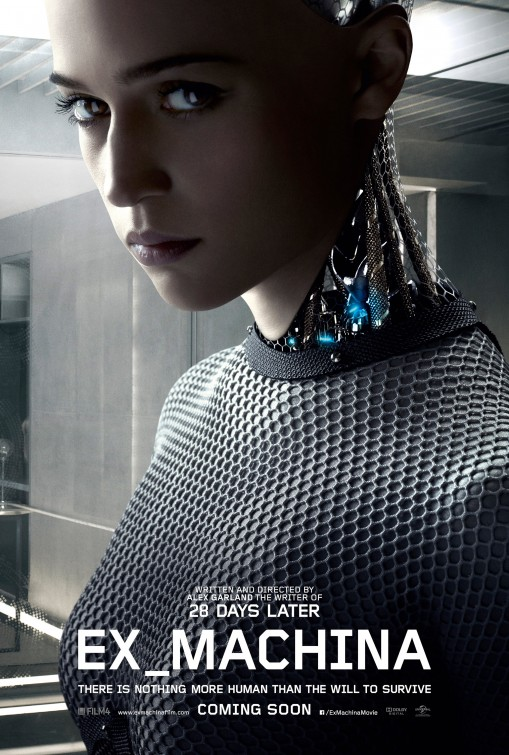
\includegraphics[width=.75\linewidth]{img/exmachina}}
    \end{center}
\end{frame}

\begin{frame}{Prerequisites}
    \begin{itemize}
        \item \textbf{What You Need}
            \begin{itemize}
                \item ability to operate a computer\\
                    (use a web browser, install software, edit text files)
                \item willingness to play around with open-ended problems
            \end{itemize}
        %
        \item \textbf{What You \highlight{WON'T} Need}
            \begin{itemize}
                \item programming experience
                \item math (except for addition, multiplication and fractions)
                \item linguistics (LIN 101 helps a bit, though)
            \end{itemize}
    \end{itemize}
\end{frame}

\begin{frame}{Three Types of Instruction}
    \begin{description}
        \item[Monday] standard lecture on language technology \\(taught by \textbf{Aniello})
        \item[Wednesday] programming sessions in Python\\  (taught by \textbf{Al{\"e}na})
        \item[Recitation] recap material with your TAs
    \end{description}

    \begin{center}
        \begin{tabular}{rccc}
                \toprule
                \textbf{Session} & \textbf{Mini-quiz?} & \textbf{Laptop?} & \textbf{Attendance?}\\
                \midrule
                Monday & yes & not recommended & recommended\\
                Wednesday & no & recommended & recommended\\
                Recitation & no & recommended & mandatory\\
                \bottomrule
        \end{tabular}
    \end{center}

    \pause
    \begin{block}{Echo Video Recordings}
        \begin{itemize}
            \item Video recordings of all lectures will be made available online.
            \item But the system is flaky, don't rely on it.
        \end{itemize}
    \end{block}
\end{frame}

\begin{frame}{Grading Components}
    \textbf{Class Participation (10\%)}
        \begin{itemize}
            \item Both in class and \highlight{online}!
            \item \textbf{Examples}:
                \begin{itemize}
                    \item ask questions
                    \item help fellow students
                    \item link to relevant online materials\\
                        $\vdots$
                \end{itemize}
            \item \textbf{Why?} 
                \begin{itemize}
                    \item Encourages you to ask questions.
                    \item Helping others is a great way of learning.
                    \item We want to have some fun, too.
                \end{itemize}
        \end{itemize}
\end{frame}

\begin{frame}{Grading Components [cont.]}
    \textbf{Mini-Quizzes (30\%)}
        \begin{itemize}
            \item at the beginning of the Monday Lectures
            \item apply techniques discussed in lecture
            \item questions template in \highlight{online quiz pool } (on CoCalc)
            \item only pass-fail grading (0 points VS 1 point)
            \item missed quiz is an automatic fail  (but 1 fail per semester is dropped)
            \item \textbf{Why?}
                \begin{itemize}
                    \item We want you to learn skills and techniques, not memorize definitions.
                                               \item Quizzes force you to self-assess how much you are getting out of the class.
                \end{itemize}
        \end{itemize}
\end{frame}

\begin{frame}{Grading Components [cont.]}
    \textbf{Python Exercises (30\%)}
        \begin{itemize}
            \item once per week
            \item programming in \highlight{Python}
            \item assigned on Wednesday at 11:59pm
            \item due the following Tuesday at 11:59pm
            \item assigned and collected through CoCalc
            \item only pass-fail grading (0 points VS 1 point)
            \item no late hand-ins (more on that later)
            \item \textbf{Why?}
                \begin{itemize}
                    \item Learning programming is like learning a new language\\
                            $\Rightarrow$ needs constant practice
                    \item Even a little bit of programming experience is incredibly useful.
                \end{itemize}
        \end{itemize}
\end{frame}


\begin{frame}{Grading Components [cont.]}
  \textbf{Midterm (30\%)}
 \begin{itemize}
            \item Tentatively in \highlight{Week 7} (during recitation)
            \item Some theory questions (like the in-class quizzes)
            \item Some pen-and-paper coding assignment        
              \item \textbf{Why?}
                \begin{itemize}
                    \item Force you to check how your study method is working, and eventually correct course
                    \item Pen-and-Paper coding helps focus on solving the problem and not on the minor details of the coding language (i.e. Python).
                \end{itemize}    
            \end{itemize}
            \textbf{Dealing with Fails}
                \begin{itemize}
        \item Optional  \highlight{Final project} for Python.
            \item Extra-credit, worth up to 20\% of the total grade
                            \item The due date for the final Python project will be announced closer to the end of the semester.
    \end{itemize}
\end{frame}

\begin{frame}{Soapbox: Thoughts on Grades}

    \begin{center}
        \begin{tabular}{cccc}
            \visible<0->{\includegraphics[width=7em]{./img/mugger1}} &
            \visible<0->{\includegraphics[width=7em]{./img/mugger2}} &
            \visible<0->{\includegraphics[width=7em]{./img/mugger3}} &
            \visible<0->{\includegraphics[width=7em]{./img/mugger4}}
        \end{tabular}
\end{center}
\pause
    \begin{itemize}
        \item Students are caught up in the \highlight{grade bubble}:
            \begin{itemize}
                \item If I get good grades I will get a job.
                \item If I get bad grades I will fail in life.
            \end{itemize}
        \item In the real world, nobody cares about your GPA.
        \item Don't focus on grades!
        \item Focus on mastering the skills you need to get the job you want.
    \end{itemize}
\end{frame}

\begin{frame}{Soapbox: Our Role in This}
    \begin{itemize}
        \item We are the academic equivalent of a \highlight{fitness trainer}.
        \item You're paying thousands of dollars for us to get you into shape,\\ and we've developed a program for you that will do that.
        \item But you are the one who has to move their body.
        \item Bad techniques like cram learning may get you a good grade,\\
              but you're cheating yourself out of true progress.
        \item If you aren't working towards long-term intellectual growth,\\
            you're flushing tons of money down the toilet.
    \end{itemize}
\end{frame}

\begin{frame}{A Note on Python }

%%        
\begin{columns}
\begin{column}{0.5\textwidth}
  \textbf{It's a steep learning curve!}
        \begin{itemize}
        \visible<2->{\item Don't despair! It takes time!}
        \end{itemize}
        \vspace{0.5cm}
          \includegraphics[width=20em]{./img/learning_curve}
\end{column}
\begin{column}{0.5\textwidth}
\visible<2->{\includegraphics[width=14em]{./img/coding}}
\end{column}
\end{columns}
\end{frame}


\begin{frame}{TL/DR: Ask for Help}
    \begin{itemize}
        \item \textbf{Take advantage of us}\\
            We put a lot of effort into helping you achieve your goals:
            %
            \begin{itemize}
                \item recitations
                \item office hours
                \item availability via email and Google hangouts
            \end{itemize}
            %
            If you don't take advantage of these opportunities,\\
            you have no right to complain about grades or homeworks. 
            
        \item \textbf{Take advantage of each other}\\
            Your peers are a valuable resource, too.
            Discuss homeworks, exchange ideas, share notes.
            Collaborate, help each other.

        \item \textbf{Don't wait too long}\\
            The Matthew effect also applies to education: the rich get richer, the poor get poorer.
            If you sense yourself falling behind, ask for help right away.
            The longer you wait, the worse it gets.
    \end{itemize}
\end{frame}

\begin{frame}{Getting Help}
    \begin{itemize}
        \item By default: use discussion forums on CoCalc
        \item We have a team of Grad and Undergrad TAs: make use of them!
            \begin{itemize}
            \item Their contacts and office hours are on Blackboard under the \textit{Instructor Info} tab.
             \end{itemize}
\end{itemize}

 \textbf{Optimizing Response Time}
  \begin{itemize}
        \item Minor technical issue? \\ $\rightarrow$ CoCalc Discussion Board > UGTA > TA > Instructors
         \item Minor/General Python Question?  \\ $\rightarrow$   CoCalc Discussion Board > UGTA > TA > Instructors
         \item Detailed Python/Homework question?  $\rightarrow$ TA > Instructors
         \item Grading question? $\rightarrow$  TA > Instructors
         \item Talked to UG TAs/TAs but still have doubts? $\rightarrow$ Instructors
         \item Personal Issues?  $\rightarrow$ Instructors
    \end{itemize}
    \end{frame}
             
 \begin{frame}{Getting Help [cont]}      
   \begin{itemize}      
        \item Contacting us:
            \begin{itemize}
                \item \textit{\{alena.aksenova,aniello.desanto\}@stonybrook.edu}
                \item Put [LIN120] at the beginning of the email \textit{Object}
                \item Reply time usually $<$ 24h (no guarantee during weekends!)
                \item If you plan to come to our office hours, drop us a line 
                    the day before.
                     \item  If there's a scheduling conflict, we'll let you know.
                    Radio silence means everything is fine.
            \end{itemize}
        \item For additional instructions, see the \emph{Getting Help} section\\
            on Blackboard.
    \end{itemize}
\end{frame}



\begin{frame}{Some Final Remarks}
    \begin{enumerate}
        \item \textbf{Course Website}
            \begin{itemize}
                \item Familiarize yourself with CoCalc and Blackboard.
                \item Lots of extra information there.
                        \item Check your SBU email frequently for Blackboard Announcements!
            \end{itemize}
        \item \textbf{Software Setup}
            \begin{itemize}
                \item We will be using mostly \highlight{CoCalc}.
                \item You will be invited to join today (via your SBU email).
                \item You have to pay a 14 dollars subscription within the first two weeks, to ensure:
                      \begin{itemize}
                      \item a fast CoCalc Virtual Machine
                      \item usable with internet connection
                      \end{itemize}
                \item More information in Wednesday lecture and in the Friday recitation.
                \item Get in touch if you have problems!
            \end{itemize}
    \end{enumerate}
\end{frame}

\begin{frame}{Supplementary Textbook (Optional!)}
    \begin{columns}
        \column{.65\linewidth}
            \begin{itemize}
                \item Al Sweigart (2015):\\
                      \emph{Automate the Boring Stuff with Python}
                \item online version \highlight{free}
                \item digital versions and hardcopy around \$25
                \item supplementary \href{https://www.youtube.com/playlist?list=PLGoJzB271_7r-iLYuEHEPJ5pSIYxXjJEn}{videos on Youtube}
                \item \highlight{It is not required}\\
                      but it's a good source to consult if something is unclear.
            \end{itemize}

        \column{.35\linewidth}
            \includegraphics[width=.9\linewidth]{./img/textbook}
    \end{columns}
\end{frame}

\begin{frame}{Tentative Schedule}
\begin{table}[]
\resizebox{\linewidth}{!}{
\begin{tabular}{ccc}
\textbf{} & \textbf{Theory} & \textbf{Python} \\ \hline
\textbf{Week 1} & Syllabus & CoCalc \& Notebook Tutorial \\ \hline
\textbf{Week 2} & Overview & Python Basics \\ \hline
\textbf{Week 3} & Overview & Strings \\ \hline
\textbf{Week 4} & Dialogue Systems & Control Flow \\ \hline
\textbf{Week 5} & Dialogue Systems & Lists \& Loops \\ \hline
\textbf{Week 6} & Word Based Models & Summary \& Practice \\ \hline
\textbf{Week 7} & More Word Based Models & Practice/Midterm \\ \hline
\textbf{Week 8} & \highlight{Spring Break} & \highlight{Spring Break} \\ \hline
\textbf{Week 9} & String Matching & String Cleaning \\ \hline
\textbf{Week 10} & N-gram Models & Functions \\ \hline
\textbf{Week 11} & Towards modern approaches: Neural Networks & Tokenizing \\ \hline
\textbf{Week 12} & Neural Networks \& Deep Learning & Ngrams \\ \hline
\textbf{Week 13} & Human-Like Models? & Frequencies \\ \hline
\textbf{Week 14} & Summary: Impact on Society & Practice/Optional Final Project \\ \hline
\end{tabular}}
\end{table}
\end{frame}

\begin{frame}{Your First Homework}
    \begin{enumerate}
        \item Carefully re-read this syllabus.
        \item Read the document \emph{How to Ace This Class} (it's on Blackboard).
        \item Create a CoCalc account and play around with ti.
         \end{enumerate}

   \textbf{Note: }There will be no mini-quiz  next Monday.  \\
    \textbf{Hint:} But in general, each week check the quiz pool online (\highlight{on CoCalc}) for example questions.
\end{frame}


\begin{frame}{Disability Support Services}
    If you have a physical, psychological, medical or learning disability that may impact your course work, please contact Disability Support Services, ECC (Educational Communications Center) Building, Room 128, (631) 632-6748. They will determine with you what accommodations, if any, are necessary and appropriate. All information and documentation is confidential.

    Students who require assistance during emergency evacuation are encouraged to discuss their needs with their professors and Disability Support Services.
    For procedures and information go to the following website:
    \url{http://www.stonybrook.edu/ehs/fire/disabilities}
\end{frame}

\begin{frame}{Academic Integrity}
    Each student must pursue his or her academic goals honestly and be personally accountable for all submitted work. Representing another person's work as your own is always wrong.  Faculty are required to report any suspected instances of academic dishonesty to the Academic Judiciary.  Faculty in the Health Sciences Center (School of Health Technology \& Management, Nursing, Social Welfare, Dental Medicine) and School of Medicine are required to follow their school-specific procedures. For more comprehensive information on academic integrity, including categories of academic dishonesty, please refer to the academic judiciary website at
    \url{http://www.stonybrook.edu/uaa/academicjudiciary/}
\end{frame}

\begin{frame}{Critical Incident Management}
    Stony Brook University expects students to respect the rights, privileges, and property of other people. Faculty are required to report to the Office of Judicial Affairs any disruptive behavior that interrupts their ability to teach, compromises the safety of the learning environment, or inhibits students' ability to learn.  Faculty in the HSC Schools and the School of Medicine are required to follow their school-specific procedures.
\end{frame}

\end{document}
